\documentclass{article}
\usepackage[T1]{fontenc}
\usepackage[utf8]{inputenc}

\usepackage[french]{babel}
\usepackage{authblk}
\usepackage{xspace}
\usepackage{graphicx,graphics} 
\usepackage{color}
\usepackage{amsmath}
\usepackage{amsfonts}
\usepackage{amssymb}
\usepackage{amsthm}
\usepackage{algorithm}
\usepackage{algorithmic}
\usepackage{longtable}
\usepackage{complexity}
\usepackage{hyperref}
\usepackage{tkz-graph}
\begin{document}

\title{Paradigmes d'ordonnancement et de routage pour l'absence de contention dans un réseau dans un context 5G et au-delà}
 

\newcommand{\todo}[1]{{\color{red} TODO: {#1}}}


\author[1,2]{\bf{ {Ma\"el Guiraud}}}
% \author[1]{Christian Cad\'er\'e}

\affil[1]{David Laboratory, UVSQ}
\affil[2]{Nokia Bell Labs France}


\maketitle

\section*{Introduction}

Avec l'arrivée de la 5G et l'augmentation du nombre d'appareils connectés, les réseaux cellulaires sont confrontés à des enjeux tels que l'augmentation de la bande passante et la diminution de la latence.

Une des technologies privilégiées par les industriels des télécoms est le C-RAN (pour Cloud Radio Access Network). Il consiste à centraliser la partie calcul (Base Band Unit en anglais, que nous appellerons BBU) des différentes antennes radio d'un secteur dans un même datacenter, afin de faciliter la maintenance et le coût d'utilisation des équipements~\cite{mobile2011c}. Le réseau d'accès entre le datacenter où se trouvent les BBU et la partie radio des antennes (Remote Radio Head, que nous appellerons RRH), s'appelle le fronthaul~\cite{ieeep802}. 

Le sujet de cette thèse nous a été proposé par Olivier Marcé et Brice Leclerc, chercheurs chez Nokia Bell Labs France. Nos travaux visent à maitriser la latence dans le fronthaul. Nous nous basons dans un premier temps sur les contraintes de temps imposées par les protocoles utilisés pour la communication entre les antennes et les mobiles pour la 4G, pour lesquels la latence de bout en bout doit être de 3ms maximum~\cite{bouguen2012lte}.  Pour la 5G, la contrainte de latence de bout en bout pourrait descendre jusqu'a 1ms~\cite{boccardi2014five}.

Nous proposons des algorithmes centralisés, qui correspondent très bien à la tendance actuelle en télécom, qui consiste à avoir un contrôleur SDN (Software Defined Network)~\cite{haleplidis2015software}, centralisant les informations et la gestion du réseau, ne laissant que peu de décision aux équipements sur la gestion de leur flux. Les flux que nous étudions sont envoyés aussi bien par les BBU que par les RRH de façon déterministe: nous considérons que les paquets envoyés ont tous la même taille, et sont envoyés périodiquement, il est donc naturel de les gérer d'une manière déterministe. L'idée de gérer de manière déterministe le réseau pour réduire la latence est populaire et explique en partie l'engouement pour le DetNet (où Deterministic Networking)~\cite{finn-detnet-architecture-08}.



  \subsection*{Encadrement et conditions de travail}
  Ma thèse CIFRE est une collaboration entre le laboratoire DAVID de l'Université de Versailles Saint-Quentin et Nokia Bell Labs France.
  Du coté académique, je suis encadré par Dominique Barth et Yann Strozecki. Olivier Marcé et Brice Leclerc sont mes référents au sein de l'entreprise. La répartition du temps de travail sur une semaine varie en fonction des objectifs et des travaux en cours, mais je ne rencontre aucune difficulté pour partager mon temps. Nous organisons des réunions mensuelles avec tous les encadrants afin de se coordonner sur les objectifs de recherche.
  
\section{Modèle}

\subsection{Modélisation par graphe et dynamique des messages}
  Nous avons choisi de modéliser le réseau comme un graphe orienté $G=(V,A)$, dans lequel les sommets représentent les noeuds du réseau et les arcs $(u,v)$ représentent les liens physiques entre ces noeuds. Ces arcs sont pondérées par un entier $\Omega(u,v)$  qui représente le temps physique pris par un message pour traverser le lien. Une {\bf route} est un chemin simple, c'est à dire une suite de sommets adjacents $u_0, \ldots , u_{l}$, avec $(u_i,u_{i+1}) \in A$. La {\bf latence} d'un sommet $u_i$ sur une route $r$ est définie par $\lambda(u_i,r)= \sum\limits_{0 \leq j <i} \Omega(u_j, u_{j+1})$. En particulier, la latence du premier sommet d'une route est $\lambda(u_0,r)=0$. La longueur d'une route $r$ est égale à  $\lambda (r)= \lambda (u_l,r)$. 
  Le premier sommet d'une route représente une RRH et le dernier sommet représente la BBU qui y est associée.
  Un {\bf réseau routé} $(G, {\cal R})$ est un graphe $G$ et un ensemble de routes dans ce graphe .
  
   \begin{figure}
       \begin{center}
      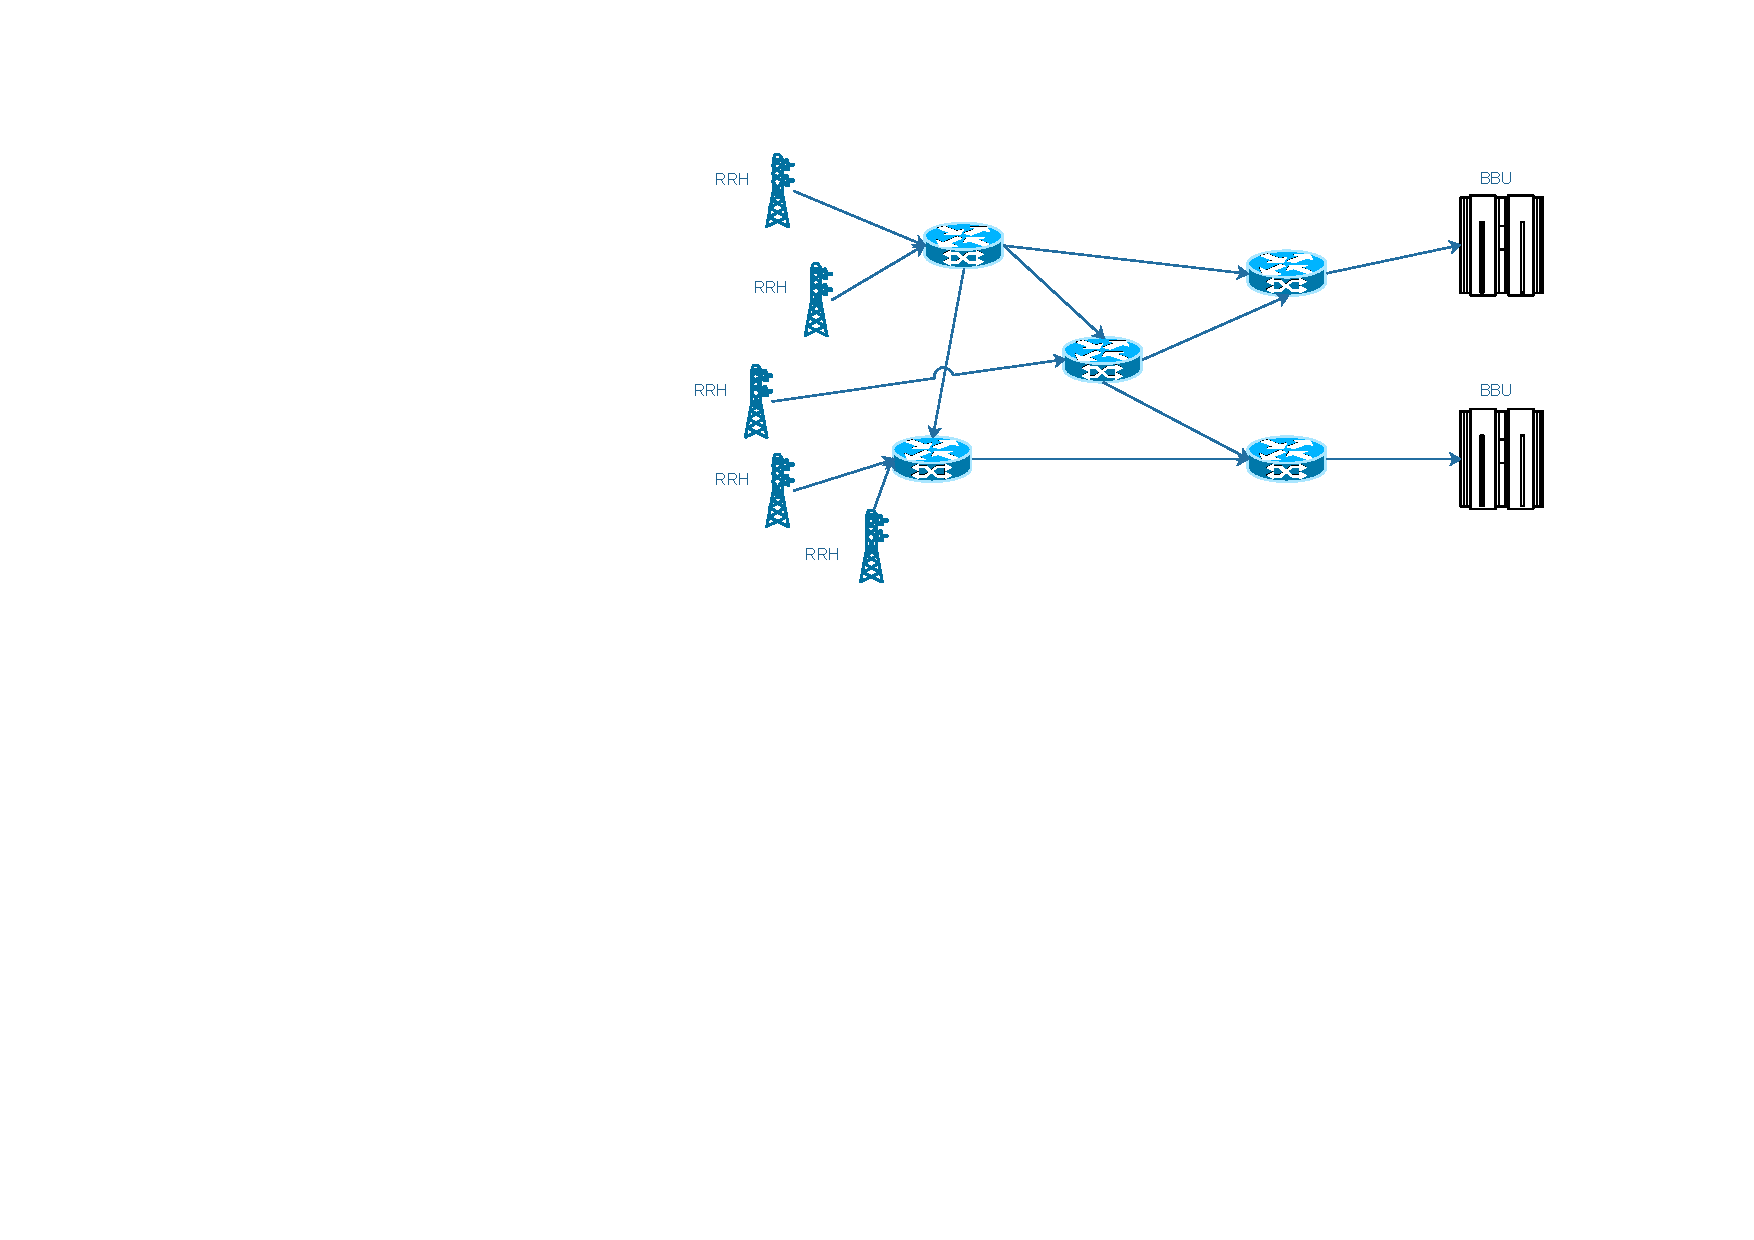
\includegraphics[width = 0.8\textwidth]{reseau.pdf}
      \end{center}
      \caption{Un exemple de réseau.}
      \label{fig:res}   
     \end{figure}    

Nous travaillons dans un modèle à temps discret. L'unité de temps est appelée le {\bf tic}, et modélise le temps nécessaire pour transmettre un paquet de $64$ octets (la plus petite taille d'un paquet en ethernet) sur un lien. La vitesse de propagation des messages dans les liens étant fixe, on peut donner le poids des arcs en tics, ce qui corresponds au temps nécéssaire à un message pour traverser le lien.
Dans les applications que nous étudions, un message est envoyé sur chaque route périodiquement. La durée de la période est notée $P$ et nous considérons que l'envoi de tout les messages ont la même périodicité.
Considérons la route $r=(u_0,\dots,u_l)$. Un message envoyé à la date $m$ de $u_0$, le premier sommet de la route $r$ arrivera au sommet $u_i$ à la date $t(u_i,r) = m + \lambda(u_i,r)$. 
Étant donné que l'envoi des messages est périodique, un message envoyé dans un arc à la date $t\in [0,P-1]$ utilisera le même arc à la date $t+kP$, pour tout $k$ entier positif. Tout les calculs peuvent donc être fait modulo $P$.

En général, les messages utilisent plus d'un tic pour être émit. La taille d'un message est notée $\tau$ et représente le nombre de tics consécutifs nécessaire pour envoyer ce message. Nous considérons que tout les messages ont la même taille.

L'ensemble des tics utilisés par un message sur une route $r$ dans l'arc $(u,v)$ est noté $[t(u,r)]_{P,\tau}$ et vaut $ \{t(u,r) + i \mod P \mid 0 \leq i < \tau \}$.
Considérons deux routes $r_1$ et $r_2$, et deux messages $m_1$ et $m_2$ envoyés respectivement du premier sommet de $r_1$ et $r_2$. Deux routes sont en {\bf conflit} si elles ont arc $(u,v)$ en commun et que $[t(u,r_{1})]_{P,\tau} \cap [t(u,r_{2})]_{P,\tau} \neq \emptyset$.
      
      
      Dans notre cas d'application du C-RAN, quand un message est envoyé depuis la RRH à la BBU, cette dernière effectue un calcul et envoie une réponse à la RRH. Dans nos travaux, un réseau routé contient deux ensembles de routes:  un ensemble de  routes aller, de chaque RRH à chaque BBU et un ensemble de routes retour, de chaque BBU à chaque RRH. Il y a une bijection $\rho$ entre les route aller et les routes retour. En général, les deux routes utilisent les mêmes arcs avec une orientation différente.
      
  Un {\bf $(P,\tau)$-periodic assignment} d'un réseau routé $(G,\cal R)$ est une fonction qui à chaque route  $r \in \cal R$ associe un {\bf offset} $m_r$, c'est à dire une date à laquelle un message est émis depuis le premier sommet de la route $r$. Dans un $(P,\tau)$-periodic assignment, \textbf{aucune paire de route n'est en conflit.}
	 
      Un assignment représente le processus suivant: un message envoyé par $u$, le premier sommet d'une route aller $r$ à la date $m_r$. Ce message est reçu par $v$, le dernier sommet de $r$ à la date $t(v,r)$. Ensuite, la réponse est envoyée par $v$ à $u$ à la date $m_{\rho(r)}$. Le temps écoulé entre l'arrivé d'un message en $v$ et l'envoi de sa réponse est appelé {\bf temps d'attente} et est défini par $w_r = m_{\rho(r)} - t(v,r)$. La figure~\ref{fig:assignment} illustre le processus d'échange de message entre une RRH et sa BBU. 
      
     \begin{figure}[h]
      \begin{center}
      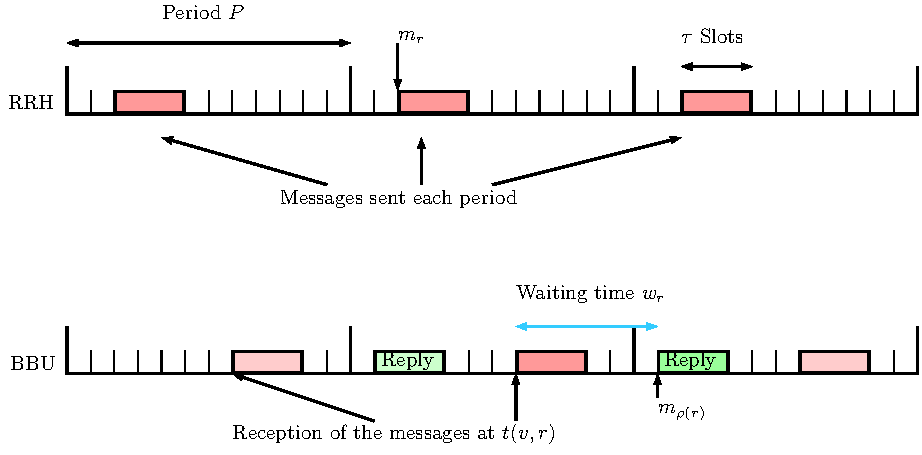
\includegraphics[width=0.8\textwidth]{rrh.pdf}
      \end{center}
      \caption{L'envoi d'un message et de sa réponse.}\label{fig:assignment}
      \end{figure}
      
Le temps de calcul avant l'envoi de la réponse n'est pas pris en compte. En effet, il est possible de considérer ce temps comme du temps de transport dans les arcs allant à la BBU afin de simplifier le problème.
      Le temps total d'aller retour d'un message envoyé sur un route $r$ est $PT(r)=\lambda(r)+ w_r+\lambda(r)$.      
      Le temps total d'aller retour de chaque route doit respecter une {\bf deadline}. Dans ce rapport, on considère la que deadline est la même pour toutes les routes et est notée $T_{max}$.
      
      Nous définissions aussi le {\bf temps de transmission} d'un réseau routé $TR(G,R) = \displaystyle \max_{i \in \{0,\ldots,n\}} t(\rho_i,u_i) - \displaystyle \min_{j \in \{0,\ldots,n\}} m_j$. C'est le temps écoulé entre l'envoi du premier message à l'aller et la réception de la dernière réponse au retour.
        
\subsection{Problèmes algorithmiques}

	Dans un premier temps, nous avons étudié un problème dans lequel les messages font un aller-retour et peuvent être mis en attente dans la BBU. Chaque message doit respecter un latence maximale. Cela correspond à des applications dans lesquelles les antennes n'ont pas besoin d'être synchrone pour envoyer et recevoir leur signaux, ce qui n'est pas possible avec les protocoles actuels. En revanche, on peut imaginer que les technologies à venir peuvent fonctionner de manière désynchronisées. De plus, ce cas de figure peut convenir à d'autres applications, comme un réseau de capteurs par exemple. Nous introduisons donc le problème suivant:

      \noindent {\bf Periodic Assignment for Low Latency (PALL)} 

      \noindent {\bf Entrées:} un réseau routé $(G,{\cal R})$, les entiers $P$, $\tau$ et $T_{max}$ .
      
      \noindent {\bf Problème de décision:} Existe-t-il un $(P,\tau)$-periodic assignment $m$ de $(G,{\cal R})$ tel que pour toute route $r \in {\cal R}$, $PT(r) \leq T_{max}$?
      
      Nous proposons aussi le problème d'optimisation suivant, dans lequel l'objectif est de minimiser la pire des latence des messages. En effet, réduire au plus possible ce temps permet d'accepter des applications de plus en plus exigeante en terme de latence.
      
       \noindent {\bf Problème d'optimisation:} Trouver un $(P,\tau)$-periodic assignment qui minimise $\displaystyle \max_{r \in R} PT(r)$.
      
      Nous avons aussi étudié un autre problème, dans lequel les BBU n'ont pas le droit d'attendre après la réception d'un message avant d'envoyer la réponse, ce qui permet d'utiliser des technologies sans file d'attente.\\
         
      \noindent {\bf Periodic Assignment for Zero Latency (PAZL)} 

      \noindent {\bf Entrée:}  Un réseau routé $(G,{\cal R})$, les entiers $P$ et $\tau$.
      
      \noindent {\bf Problème de décision:} Existe-t-il un assignment $m$ de $(G,{\cal R})$, dans lequel $w_r = 0$ pour toute route $r \in {\cal R}$.

Dans le cas d'application du C-RAN, les antennes envoient leurs messages de façon synchronisée, c'est à dire au même tic à chaque période. Ensuite, toutes les réponses doivent revenir aux  antennes avant une deadline générale.
Nous définissions donc le problème suivant :
       
       \noindent {\bf Synchronized Periodic Assignment for Low Latency (SPALL) } 

      \noindent {\bf Entrées :}  Un réseau routé $(G,{\cal R})$, les entiers $P$, $Tmax$.
      
      \noindent {\bf Problème de décision:} Existe-t-il un assignment $m$ de $(G,{\cal R})$ tel que $ TR(G,{\cal R}) \leq Tmax$ ?

      \noindent {\bf Problème d'optimisation:} Trouver un $(P,\tau)$-periodic assignment qui minimise  $TR(G,{\cal R})$.
    
Dans le cas ou les antennes sont synchronisées, il n'est pas pertinent de chercher des assignments avec zéro temps d'attente, car ça n'a pas d'impact sur la mesure que nous cherchons à optimiser, en l'occurence $TR(G,{\cal R})$.

Il apparait que les problèmes exposés ressemblent à des problèmes d'ordonnancement. En revanche, la périodicité des messages nous empêche de réduire notre problème à un problème d'ordonnancement classique.
  
\section{Topologies étudiées}
Nous définissons la {\bf profondeur de conflit} d'une route comme le nombre d'arc que cette route partage avec d'autres routes.

  \subsection{Réseau sous forme d'étoile: profondeur de conflit $1$}
	
	
Dans un premier temps, pendant mon stage de master et le début de ma thèse, nous avons étudié un réseau sous forme d'étoile. C'est un réseau réaliste qui correspond à des architectures Point-to-Multipoint (PtMP), assez courantes dans le C-RAN \cite{tayq2017real}. 
Le graphe $G$ comprend deux ensembles de sommets $S=\{s_0,...,s_{n-1}\}$ et $T=\{t_0,...,t_{n-1}\}$ de taille $n$ et deux sommets spéciaux: {\bf $c_s$} (pour central sources) et {\bf $c_t$} (pour central target).
    Il y a un arc entre {\bf $c_s$} et {\bf $c_t$} et pour chaque route $i$, il y a un arc entre $s_i$ et $c_s$ et entre $t_i$ et $c_t$.
      Les routes sont les chemins $r_i = (s_i,c_s,c_t,t_i)$ à l'aller et  $\rho(r_i) = (t_i,c_t,c_s,s_i)$ au retour. 
      Ce genre de topologie peut paraître simple, mais nous avons pu prouver que le problème SPALL est NP-complet~\cite{orman1997complexity}, même sur cette topologie, et nous suspectons que les problèmes PAZL et PALL le sont aussi car des variantes dans lequel le lien central est partagé le sont~\cite{yu2004minimizing}. Dans la prochaine section nous verrons quelques algorithmes gloutons et FPT qui permettent d'obtenir de bonnes solutions pour ces trois problèmes sur cette topologie.
      \begin{figure}
       \begin{center}
	 \scalebox{0.8}{
\begin{tikzpicture}

\tikzset{EdgeStyle/.style={<->,font=\scriptsize,above,sloped,midway}}
  \SetGraphUnit{5}
  
  \node[draw,circle] (s3) at (0, 0) {$s_2$}; 
  \node[draw,circle] (s2) at (0, 2) {$s_1$}; 
  \node[draw,circle] (s1) at (0, 4) {$s_0$}; 

  \node[draw,circle] (t3) at (8, 0) {$t_2$}; 
  \node[draw,circle] (t2) at (8, 2) {$t_1$}; 
  \node[draw,circle] (t1) at (8, 4) {$t_0$}; 
  

  \node[draw,circle] (cs) at (3, 2) {$c_s$}; 
  \node[draw,circle] (ct) at (5, 2) {$c_t$}; 

  
  \Edge[label = $\Omega(s_0\,c_s)$](s1)(cs)
  \Edge[label = $\Omega(...)$](s2)(cs)
  \Edge[label = $\Omega(...)$](s3)(cs)
  
  \Edge[label = $\Omega(...)$](ct)(t1)
  \Edge[label = $\Omega(...)$](ct)(t2)
  \Edge[label = $\Omega(...)$](ct)(t3)
  
  \Edge(cs)(ct)

  
\end{tikzpicture}
}

  \end{center}
  \caption{Réseau sous forme d'étoile}
  \end{figure}
  
  Nous avons proposé plusieurs solutions pour les problèmes PAZL et PALL pour cette topologie, les résultats ont été présentés à la conférence ICT 2018~\cite{DBLP:conf/ict/BarthGLMS18}, et une version longue à été soumise au journal TCS~\cite{DBLP:journals/corr/abs-1902-03018}.
  \subsection{Anneau optique}
  J'ai travaillé avant le début de ma thèse pour le projet ANR NGREEN, pour lequel j'ai été amené à étudier le comportement du traffic C-RAN sur un anneau optique novateur~\cite{ngreenarchitecture,uscumlic2018scalable}.
  Après modélisation de l'anneau et de sa technologie et définition du problème algorithmique d'organisation des flux déterministes entre eux, nous nous sommes aperçu que notre problème était trivial en raison des paramètres spécifiques de l'architecture. Néanmoins, l'interface entre le réseau électronique et le réseau optique était une nouveauté qu'il a fallu modéliser correctement pour bien résoudre le problème. De plus, nous avons proposé des solutions pour organiser nos flux prioritaires de façon à impacter le moins possible la latence des flux dit "best effort". J'ai présenté ces résultats sous forme de poster à la conférence ONDM 2019~\cite{DBLP:journals/corr/abs-1902-03018}. Suite à nos travaux, il s'avère que le fait d'organiser correctement les flux déterministes aide même à réduire la latence des flux best effort.

   \subsection{Topologie plus générale: profondeur de conflit $2$}
 
 Après avoir beaucoup étudié la topologie de profondeur $1$, nous nous sommes penchés sur une topologie plus générale, tout en restant sur des réseaux réalistes. Nous avons naturellement choisi de regarder des DAG de profondeur de conflit $2$, c'est à dire dans lesquels une route n'a que deux arcs sur lesquels elle est en conflit avec les autres routes.
 La figure~\ref{fig:extendendgraphgrey} représente le type de réseau que nous étudions. 

\begin{figure}[h]
\begin{center}
 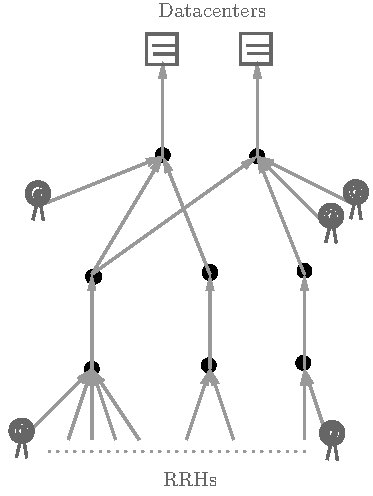
\includegraphics[width=0.4\textwidth]{extendendgraphgrey}
\caption{Un réseau de profondeur de conflit $2$.}\label{fig:extendendgraphgrey}
\end{center}
\end{figure}
\section{Solutions algorithmiques pour l'étoile.}

Nous définissons la {\bf charge} du réseau comme le rapport entre le nombre de tics nécessaire pour faire passer les messages de toutes les routes et le nombre de tics d'une période.

\subsection{PAZL}
 Nous avons dans un premier temps choisi d'étudier le problème PAZL, dans lequel toutes les solutions trouvées seraient optimales en latence.
 
 Dans un premier temps nous proposons plusieurs algorithmes gloutons.
 \begin{itemize}
 \item Un algorithme glouton qui nous assure de trouver une solution si la charge du réseau est est inférieure à $1/3$. Cet algorithme (Greedy dans la figure~\ref{fig:long}) fonctionne de la manière suivante: pour chaque route, on attribue le premier temps de départ disponible qui ne crée pas de conflit avec les routes déjà placées.
 \item  Nous avons aussi prouvé que si la différence entre la taille des routes est suffisamment petite par rapport à la période, il existe une solution au problème PAZL. Dans ce cas, on trie les routes par ordre croissant de taille et on envoie les messages à la suite dans l'arc central à l'aller, de celui qui utilise la route la plus courte à celui qui utilise la route la plus longe. Nous appelons cet algorithme Shortest Longest
 \item Nous proposons également un algorithme de recherche exhaustive de complexité FPT en $n$ le nombre de routes, ce qui est interessant car le nombre de route est le paramètre le plus petit de nos instances. L'idée de l'algorithme est de décrire une solution sous une forme normale dans laquelle les messages sont collées entre eux soit à l'aller, soit au retour, et de tester tout les ordres possibles des messages à l'aller et au retour.
 \end{itemize}
 
 Nous avons simulé le comportement de nos algorithmes sur des graphes aléatoires avec des routes dont la longueur est soit petite par rapport à la période soit longue. \begin{itemize}
 \item Dans le cas de routes courtes, organiser les routes de la plus courte à la plus longue donne presque toujours la solution optimale.
 \item Dans le cas de routes longues, nous avons comparé nos deux heuristiques à l'algorithme FPT. Dans ce cas, trier les routes dans l'ordre donne une mauvaise solution et
 l'algorithme glouton fonctionne bien jusqu'à $50\%$ de charge. La recherche exhaustive montre qu'il existe presque toujours une solution jusqu'à $80\%$ de charge et qu'il y en a rarement pour les charges plus élevées.
  \end{itemize}     
  
 La figure~\ref{fig:long} représente les performances des algorithmes que nous venons de présenter, sur des instances avec des routes longues.
\begin{figure}[h]

       \begin{center}
      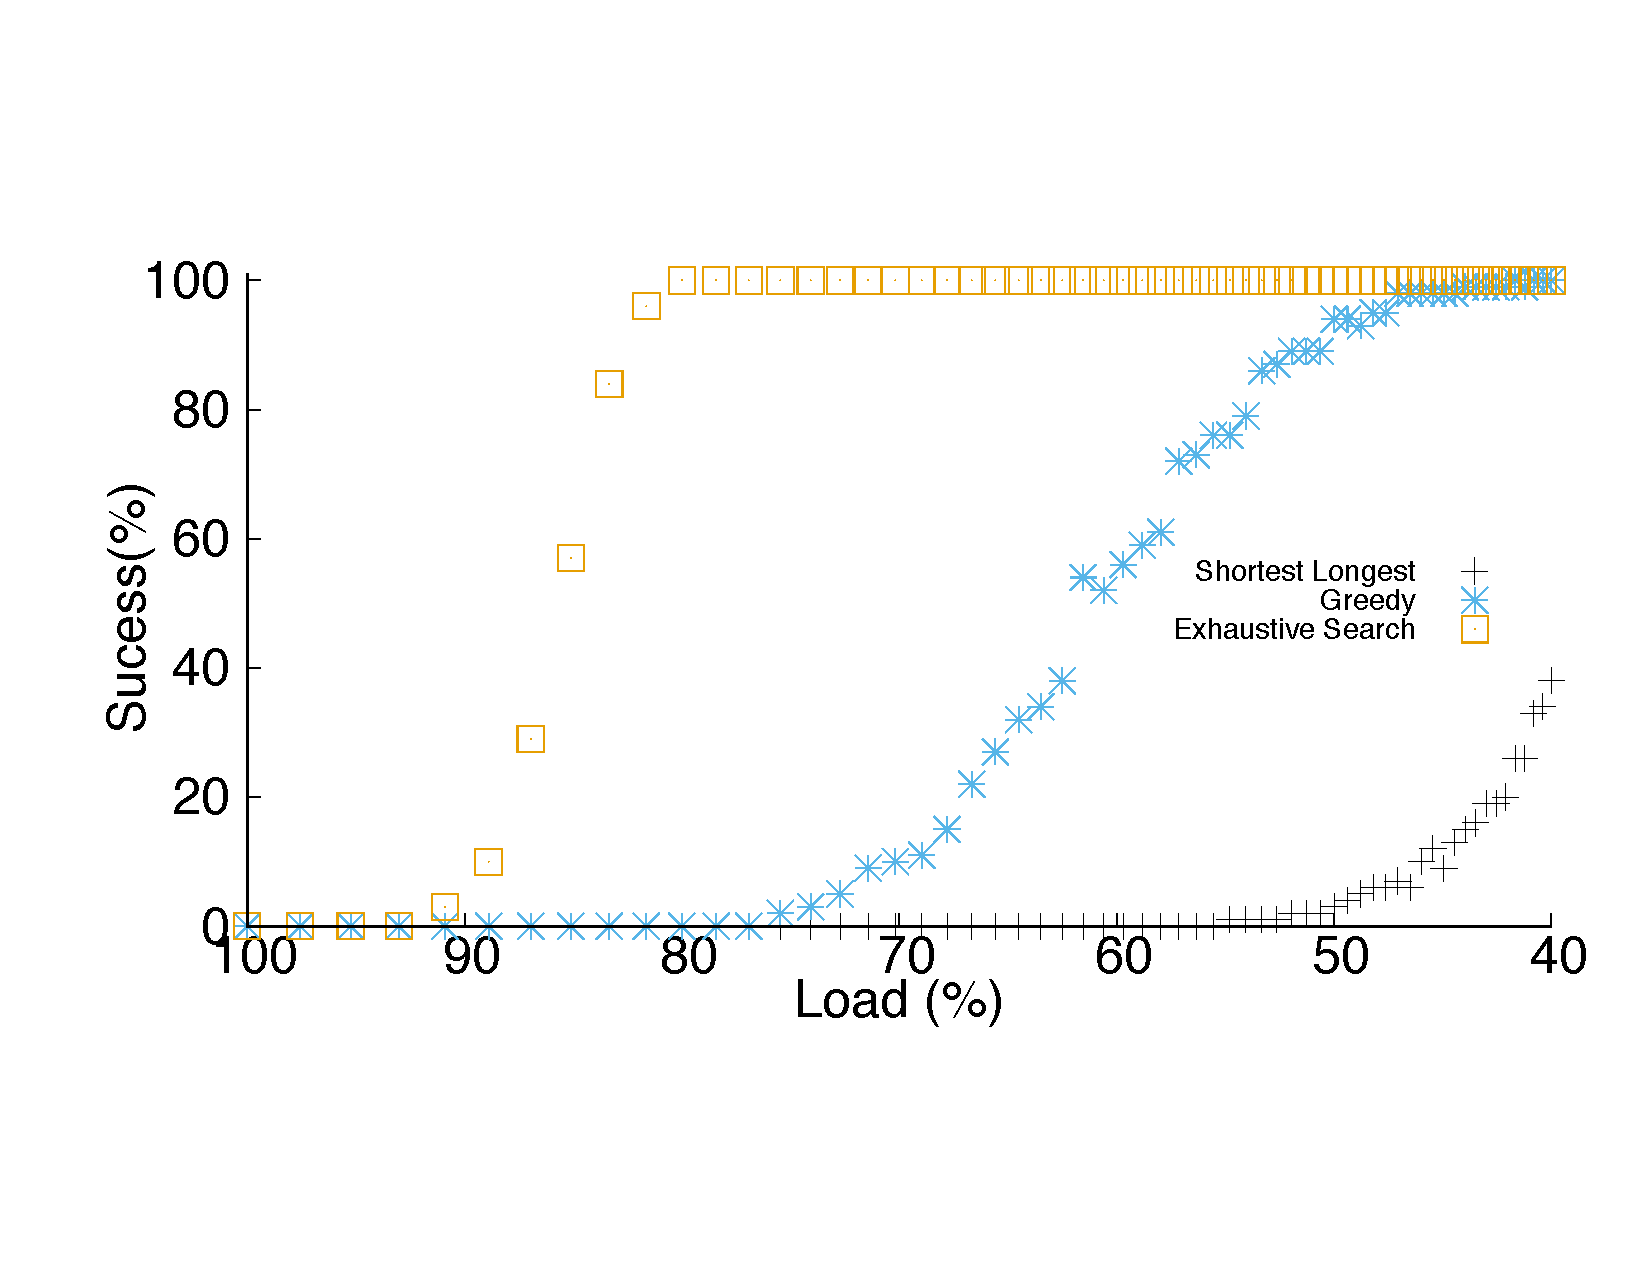
\includegraphics[width=0.8\textwidth]{echec_longues.pdf}
      \end{center}
       
      \caption{Taux de réussite des algorithmes en fonction de la charge.}\label{fig:long}
     \end{figure}
     
\subsection{PALL}
Étant donné qu'il n'existe pas de solution sans temps d'attente quand la charge est élevée, nous nous sommes intéressés au problème PALL qui permet un temps d'attente dans les BBU. Ce problème nous offre une plus grande liberté, en effet, nous nous autorisons à dégrader la latence de certains messages pour pouvoir trouver des solutions dans lesquelles la condition de latence globale est satisfaite.

Nos algorithmes pour résoudre ce problème peuvent se décomposer en deux phases. D'abord on fixe la phase aller, de façon arbitraire, puis on essaye d'organiser les messages au retour. Dans ce cas, on obtiens un problème avec en entrée un temps de départ minimal pour chaque route, une date limite d'envoi et une taille de message. Si on ne considère pas la périodicité, c'est un problème d'ordonnancement classique de "single processor scheduling" dans lequel les tâches ont la même durée. Il existe un algorithme polynomial~\cite{simons1978fast} qui trouve une solution à ce problème en minimisant le temps de complétion. Nous appellerons cet algorithme MLS.

Cet algorithme ne donnait toujours pas de bonnes performances, car il ne prend pas la périodicité du problème PALL en compte. Nous proposons deux méthodes pour intégrer la périodicité à l'algorithme MLS.
\begin{itemize}
\item La première solution (PMLS) est de modifier les dates limites des routes pour faire en sorte que tous les messages soient ordonnancés dans la même période.
\item La seconde solution (FPT-PMLS) est un algorithme FPT en le nombre de routes qui devine dans quelle période on fait passer un messages entre deux périodes consécutives. Cet algorithme nous donne une solution optimale pour le problème du retour.
\end{itemize}
Nous avons également proposé un algorithme glouton (GD pour Greedy Deadline) qui organise les messages selon leur dates limites. 

La figure~\ref{fig:success21000} représente les performances de différents algorithmes que nous proposons. Notre algorithme glouton adapté pour la périodicité (GD), l'algorithme d'ordonnancement qui ne gère pas du tout la périodicité (MLS), adapté pour la périodicité (PMLS), et l'algorithme FPT (FPT-PMLS).
Pour chaque instance, nous fixons la latence maximal à deux fois la taille de la route la plus longue, puis nous avons fait varier la margin, qui correspond à du temps de latence supplémentaire donné aux messages.

    \begin{figure} [h] 
       \begin{center}
      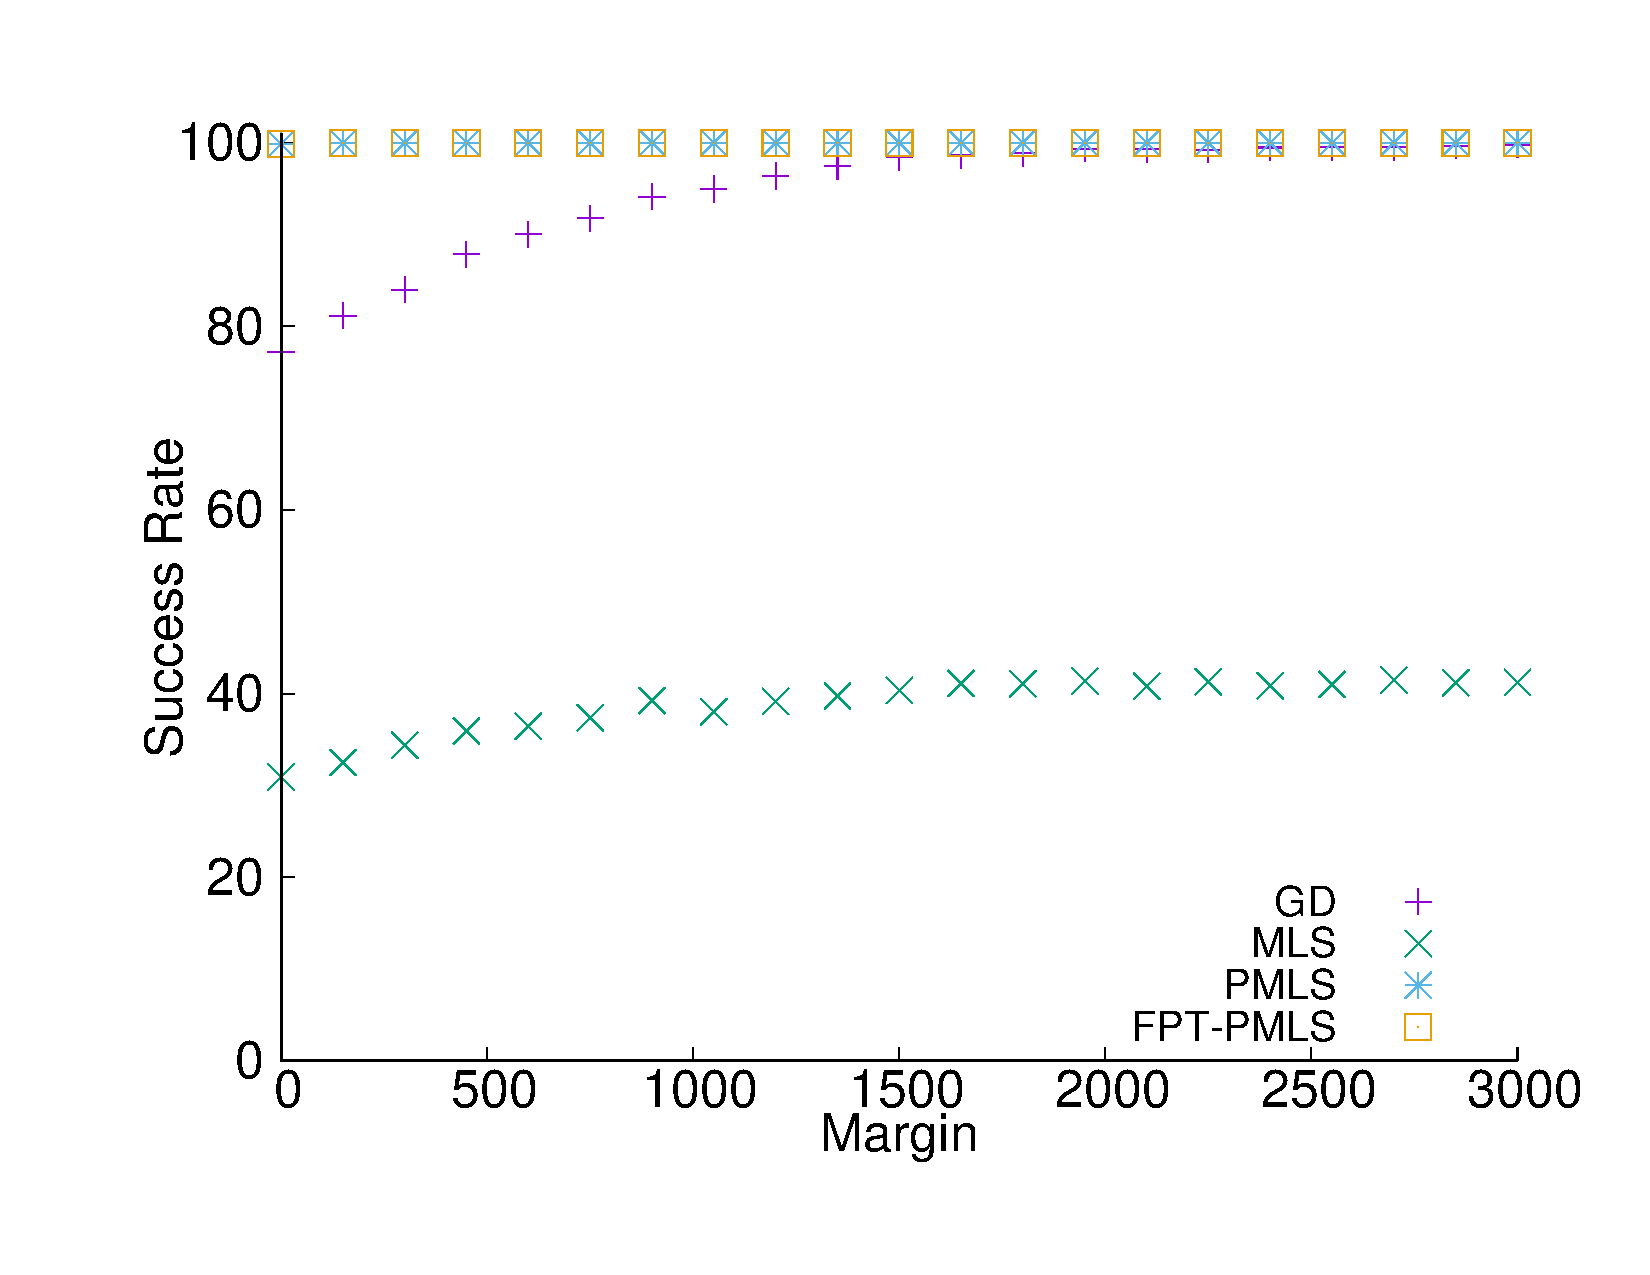
\includegraphics[width=0.8\textwidth]{retour_21000.pdf}
      \end{center}
      \caption{Taux de réussite des algorithmes pour le retour, à $95\%$ de charge.}
     \label{fig:success21000}
     \end{figure}
    
    Les deux algorithmes (PMLS et FPT PMLS ) présentent d'excellentes performances, même sur un réseau très chargé.
  En pratique l'algorithme FPT ne trouve pas beaucoup plus de solutions que PMLS. En effet, il y à très peu d'instances pour lesquelles il est utile d'utiliser l'algorithme FPT.
  Il est donc recommandé d'utiliser l'algorithme PMLS, surtout quand il y a beaucoup de routes (calcul $15000$ fois plus long avec l'algorithme FPT pour $24$ routes). Il est important de noter que la gestion de la périodicité est capitale dans notre problème. En effet, l'algorithme MLS ne trouve que très peu de solution par rapport à notre algorithme glouton qui prend en compte la périodicité.

Afin de fixer l'ordre et la date de départ des temps à l'aller, nous avons essayé plusieurs variantes. Nous avons essayé différents ordres: envoyer les messages sur les routes de la plus longue a la plus courte, de la route la plus courte à la plus longue, où de les envoyer dans un ordre aléatoire. En ce qui concerne les dates de départ, nous avons essayé de coller tout les messages, et d'espacer les messages de façon uniforme, où aléatoire dans la période. Finalement, après des simulations, nous avons conclu que la meilleure façon de trouver une solution pour le problème PALL est de générer un grand nombre d'ordres aléatoires, de coller tout les messages à l'aller et de chercher une solution pour le retour avec l'algorithme PMLS.

Nous avons aussi proposé un algorithme FPT pour le problème PALL (aller et retour). À une instance on associe un nombre exponentiel (qui dépend du nombre de routes) de système linéaires tels que si l'un au moins d'entre eux est satisfait, il existe une solution. Nous ne l'avons pas implémenté car ses performances ne permettraient pas de traiter plus de quelques solutions et que l'algorithme précédent nous permet déjà de trouver un très grand nombre de solutions d'excellentes qualités. Néanmoins, ayant trouvé des papiers récents en rapport avec nos travaux, nous avons contacté plusieurs équipes qui utilisent la programmation linéaire pour résoudre un problème très similaire au notre, afin de collaborer et de confronter nos travaux respectifs~\cite{steiner2018traffic,craciunas2017formal}.


     
\subsection{SPALL}
Le problème SPALL est en fait une variante plus simple de PALL sur l'étoile. Étant donné que le temps est compté dès l'envoi du message depuis la RRH, il n'y a pas d'intérêt à retarder les messages dans la RRH. Pour choisir comment envoyer les routes à l'aller, il suffit donc de choisir l'ordre d'envoi des routes. Ensuite, nous pouvons utiliser l'algorithme FPT utilisé pour PALL au retour. Nous avons donc un algorithme FPT pour résoudre le problème SPALL sur l'étoile qui est efficace en pratique pour $20$ routes contrairement à celui proposé pour PALL.



\subsection{Comparaison avec une gestion statistique des messages}
Afin d'évaluer les performances de nos algorithmes d'organisation déterministe des flux dans les réseaux, nous avons choisis d'implémenter un simulateur du comportement actuel des réseaux. Tout les messages sont envoyés dès qu'ils sont disponibles, et si ils doivent utiliser un même lien en même temps, alors l'un des deux est mis dans une file d'attente dans le noeud de départ de ce lien en attendant qu'il puisse utiliser la ressource partagée. Nous avons étudié deux politiques de gestion de message dans les files d'attentes en cas de conflit. La première est le FIFO basique, et la seconde est d'envoyer le message qui à arriverait le plus tard à sa destination. 
La figure~\ref{fig:sto} représente les performances de notre algorithme PMLS, comparé à une gestion statistique des flux.
 \begin{figure}
       \begin{center}
      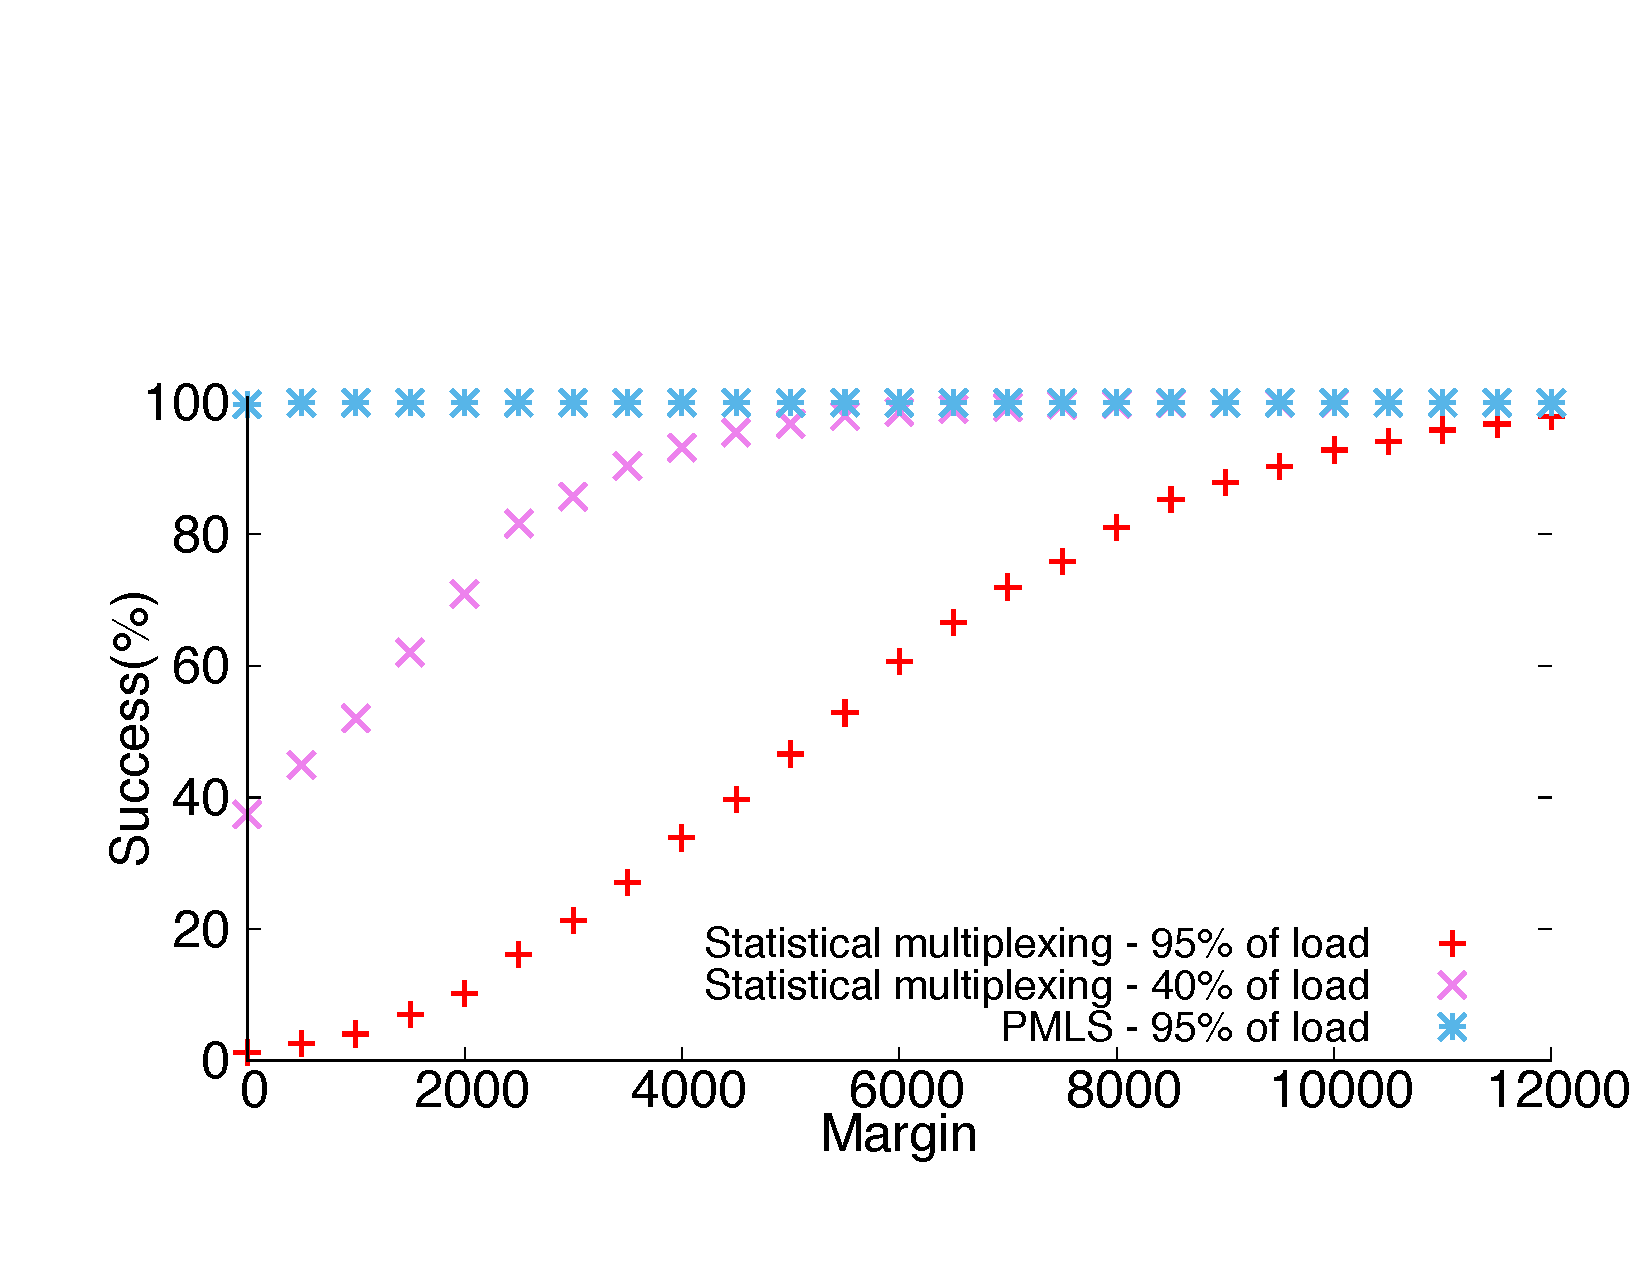
\includegraphics[width = 0.8\textwidth]{stochastic.pdf}
       %% GNUPLOT: LaTeX picture
\setlength{\unitlength}{0.240900pt}
\ifx\plotpoint\undefined\newsavebox{\plotpoint}\fi
\sbox{\plotpoint}{\rule[-0.200pt]{0.400pt}{0.400pt}}%
\begin{picture}(1500,900)(0,0)
\sbox{\plotpoint}{\rule[-0.200pt]{0.400pt}{0.400pt}}%
\put(171.0,131.0){\rule[-0.200pt]{4.818pt}{0.400pt}}
\put(151,131){\makebox(0,0)[r]{$0$}}
\put(1279.0,131.0){\rule[-0.200pt]{4.818pt}{0.400pt}}
\put(171.0,212.0){\rule[-0.200pt]{4.818pt}{0.400pt}}
\put(151,212){\makebox(0,0)[r]{$1000$}}
\put(1279.0,212.0){\rule[-0.200pt]{4.818pt}{0.400pt}}
\put(171.0,293.0){\rule[-0.200pt]{4.818pt}{0.400pt}}
\put(151,293){\makebox(0,0)[r]{$2000$}}
\put(1279.0,293.0){\rule[-0.200pt]{4.818pt}{0.400pt}}
\put(171.0,374.0){\rule[-0.200pt]{4.818pt}{0.400pt}}
\put(151,374){\makebox(0,0)[r]{$3000$}}
\put(1279.0,374.0){\rule[-0.200pt]{4.818pt}{0.400pt}}
\put(171.0,455.0){\rule[-0.200pt]{4.818pt}{0.400pt}}
\put(151,455){\makebox(0,0)[r]{$4000$}}
\put(1279.0,455.0){\rule[-0.200pt]{4.818pt}{0.400pt}}
\put(171.0,535.0){\rule[-0.200pt]{4.818pt}{0.400pt}}
\put(151,535){\makebox(0,0)[r]{$5000$}}
\put(1279.0,535.0){\rule[-0.200pt]{4.818pt}{0.400pt}}
\put(171.0,616.0){\rule[-0.200pt]{4.818pt}{0.400pt}}
\put(151,616){\makebox(0,0)[r]{$6000$}}
\put(1279.0,616.0){\rule[-0.200pt]{4.818pt}{0.400pt}}
\put(171.0,697.0){\rule[-0.200pt]{4.818pt}{0.400pt}}
\put(151,697){\makebox(0,0)[r]{$7000$}}
\put(1279.0,697.0){\rule[-0.200pt]{4.818pt}{0.400pt}}
\put(171.0,778.0){\rule[-0.200pt]{4.818pt}{0.400pt}}
\put(151,778){\makebox(0,0)[r]{$8000$}}
\put(1279.0,778.0){\rule[-0.200pt]{4.818pt}{0.400pt}}
\put(171.0,859.0){\rule[-0.200pt]{4.818pt}{0.400pt}}
\put(151,859){\makebox(0,0)[r]{$9000$}}
\put(1279.0,859.0){\rule[-0.200pt]{4.818pt}{0.400pt}}
\put(171.0,131.0){\rule[-0.200pt]{0.400pt}{4.818pt}}
\put(171,90){\makebox(0,0){$20000$}}
\put(171.0,839.0){\rule[-0.200pt]{0.400pt}{4.818pt}}
\put(359.0,131.0){\rule[-0.200pt]{0.400pt}{4.818pt}}
\put(359,90){\makebox(0,0){$25000$}}
\put(359.0,839.0){\rule[-0.200pt]{0.400pt}{4.818pt}}
\put(547.0,131.0){\rule[-0.200pt]{0.400pt}{4.818pt}}
\put(547,90){\makebox(0,0){$30000$}}
\put(547.0,839.0){\rule[-0.200pt]{0.400pt}{4.818pt}}
\put(735.0,131.0){\rule[-0.200pt]{0.400pt}{4.818pt}}
\put(735,90){\makebox(0,0){$35000$}}
\put(735.0,839.0){\rule[-0.200pt]{0.400pt}{4.818pt}}
\put(923.0,131.0){\rule[-0.200pt]{0.400pt}{4.818pt}}
\put(923,90){\makebox(0,0){$40000$}}
\put(923.0,839.0){\rule[-0.200pt]{0.400pt}{4.818pt}}
\put(1111.0,131.0){\rule[-0.200pt]{0.400pt}{4.818pt}}
\put(1111,90){\makebox(0,0){$45000$}}
\put(1111.0,839.0){\rule[-0.200pt]{0.400pt}{4.818pt}}
\put(1299.0,131.0){\rule[-0.200pt]{0.400pt}{4.818pt}}
\put(1299,90){\makebox(0,0){$50000$}}
\put(1299.0,839.0){\rule[-0.200pt]{0.400pt}{4.818pt}}
\put(171.0,131.0){\rule[-0.200pt]{0.400pt}{175.375pt}}
\put(171.0,131.0){\rule[-0.200pt]{271.735pt}{0.400pt}}
\put(30,495){\makebox(0,0){Needed Flexibility}}
\put(735,29){\makebox(0,0){Period}}
\put(171.0,455.0){\rule[-0.200pt]{0.400pt}{81.183pt}}
\put(171.0,455.0){\rule[-0.200pt]{2.409pt}{0.400pt}}
\put(171.0,792.0){\rule[-0.200pt]{2.409pt}{0.400pt}}
\put(209.0,412.0){\rule[-0.200pt]{0.400pt}{73.715pt}}
\put(199.0,412.0){\rule[-0.200pt]{4.818pt}{0.400pt}}
\put(199.0,718.0){\rule[-0.200pt]{4.818pt}{0.400pt}}
\put(246.0,353.0){\rule[-0.200pt]{0.400pt}{79.497pt}}
\put(236.0,353.0){\rule[-0.200pt]{4.818pt}{0.400pt}}
\put(236.0,683.0){\rule[-0.200pt]{4.818pt}{0.400pt}}
\put(284.0,336.0){\rule[-0.200pt]{0.400pt}{75.883pt}}
\put(274.0,336.0){\rule[-0.200pt]{4.818pt}{0.400pt}}
\put(274.0,651.0){\rule[-0.200pt]{4.818pt}{0.400pt}}
\put(321.0,306.0){\rule[-0.200pt]{0.400pt}{70.343pt}}
\put(311.0,306.0){\rule[-0.200pt]{4.818pt}{0.400pt}}
\put(311.0,598.0){\rule[-0.200pt]{4.818pt}{0.400pt}}
\put(359.0,297.0){\rule[-0.200pt]{0.400pt}{73.715pt}}
\put(349.0,297.0){\rule[-0.200pt]{4.818pt}{0.400pt}}
\put(349.0,603.0){\rule[-0.200pt]{4.818pt}{0.400pt}}
\put(397.0,270.0){\rule[-0.200pt]{0.400pt}{63.598pt}}
\put(387.0,270.0){\rule[-0.200pt]{4.818pt}{0.400pt}}
\put(387.0,534.0){\rule[-0.200pt]{4.818pt}{0.400pt}}
\put(434.0,269.0){\rule[-0.200pt]{0.400pt}{64.561pt}}
\put(424.0,269.0){\rule[-0.200pt]{4.818pt}{0.400pt}}
\put(424.0,537.0){\rule[-0.200pt]{4.818pt}{0.400pt}}
\put(472.0,238.0){\rule[-0.200pt]{0.400pt}{69.138pt}}
\put(462.0,238.0){\rule[-0.200pt]{4.818pt}{0.400pt}}
\put(462.0,525.0){\rule[-0.200pt]{4.818pt}{0.400pt}}
\put(509.0,226.0){\rule[-0.200pt]{0.400pt}{62.393pt}}
\put(499.0,226.0){\rule[-0.200pt]{4.818pt}{0.400pt}}
\put(499.0,485.0){\rule[-0.200pt]{4.818pt}{0.400pt}}
\put(547.0,222.0){\rule[-0.200pt]{0.400pt}{60.225pt}}
\put(537.0,222.0){\rule[-0.200pt]{4.818pt}{0.400pt}}
\put(537.0,472.0){\rule[-0.200pt]{4.818pt}{0.400pt}}
\put(585.0,195.0){\rule[-0.200pt]{0.400pt}{60.225pt}}
\put(575.0,195.0){\rule[-0.200pt]{4.818pt}{0.400pt}}
\put(575.0,445.0){\rule[-0.200pt]{4.818pt}{0.400pt}}
\put(622.0,185.0){\rule[-0.200pt]{0.400pt}{58.780pt}}
\put(612.0,185.0){\rule[-0.200pt]{4.818pt}{0.400pt}}
\put(612.0,429.0){\rule[-0.200pt]{4.818pt}{0.400pt}}
\put(660.0,178.0){\rule[-0.200pt]{0.400pt}{59.743pt}}
\put(650.0,178.0){\rule[-0.200pt]{4.818pt}{0.400pt}}
\put(650.0,426.0){\rule[-0.200pt]{4.818pt}{0.400pt}}
\put(697.0,188.0){\rule[-0.200pt]{0.400pt}{59.020pt}}
\put(687.0,188.0){\rule[-0.200pt]{4.818pt}{0.400pt}}
\put(687.0,433.0){\rule[-0.200pt]{4.818pt}{0.400pt}}
\put(735.0,152.0){\rule[-0.200pt]{0.400pt}{55.889pt}}
\put(725.0,152.0){\rule[-0.200pt]{4.818pt}{0.400pt}}
\put(725.0,384.0){\rule[-0.200pt]{4.818pt}{0.400pt}}
\put(773.0,146.0){\rule[-0.200pt]{0.400pt}{57.575pt}}
\put(763.0,146.0){\rule[-0.200pt]{4.818pt}{0.400pt}}
\put(763.0,385.0){\rule[-0.200pt]{4.818pt}{0.400pt}}
\put(810.0,146.0){\rule[-0.200pt]{0.400pt}{54.925pt}}
\put(800.0,146.0){\rule[-0.200pt]{4.818pt}{0.400pt}}
\put(800.0,374.0){\rule[-0.200pt]{4.818pt}{0.400pt}}
\put(848.0,143.0){\rule[-0.200pt]{0.400pt}{56.371pt}}
\put(838.0,143.0){\rule[-0.200pt]{4.818pt}{0.400pt}}
\put(838.0,377.0){\rule[-0.200pt]{4.818pt}{0.400pt}}
\put(885.0,140.0){\rule[-0.200pt]{0.400pt}{56.371pt}}
\put(875.0,140.0){\rule[-0.200pt]{4.818pt}{0.400pt}}
\put(875.0,374.0){\rule[-0.200pt]{4.818pt}{0.400pt}}
\put(923.0,133.0){\rule[-0.200pt]{0.400pt}{54.202pt}}
\put(913.0,133.0){\rule[-0.200pt]{4.818pt}{0.400pt}}
\put(913.0,358.0){\rule[-0.200pt]{4.818pt}{0.400pt}}
\put(961.0,131.0){\rule[-0.200pt]{0.400pt}{55.166pt}}
\put(951.0,131.0){\rule[-0.200pt]{4.818pt}{0.400pt}}
\put(951.0,360.0){\rule[-0.200pt]{4.818pt}{0.400pt}}
\put(998.0,131.0){\rule[-0.200pt]{0.400pt}{49.384pt}}
\put(988.0,131.0){\rule[-0.200pt]{4.818pt}{0.400pt}}
\put(988.0,336.0){\rule[-0.200pt]{4.818pt}{0.400pt}}
\put(1036.0,131.0){\rule[-0.200pt]{0.400pt}{48.180pt}}
\put(1026.0,131.0){\rule[-0.200pt]{4.818pt}{0.400pt}}
\put(1026.0,331.0){\rule[-0.200pt]{4.818pt}{0.400pt}}
\put(1073.0,131.0){\rule[-0.200pt]{0.400pt}{47.216pt}}
\put(1063.0,131.0){\rule[-0.200pt]{4.818pt}{0.400pt}}
\put(1063.0,327.0){\rule[-0.200pt]{4.818pt}{0.400pt}}
\put(1111.0,131.0){\rule[-0.200pt]{0.400pt}{46.975pt}}
\put(1101.0,131.0){\rule[-0.200pt]{4.818pt}{0.400pt}}
\put(1101.0,326.0){\rule[-0.200pt]{4.818pt}{0.400pt}}
\put(1149.0,131.0){\rule[-0.200pt]{0.400pt}{45.048pt}}
\put(1139.0,131.0){\rule[-0.200pt]{4.818pt}{0.400pt}}
\put(1139.0,318.0){\rule[-0.200pt]{4.818pt}{0.400pt}}
\put(1186.0,131.0){\rule[-0.200pt]{0.400pt}{46.494pt}}
\put(1176.0,131.0){\rule[-0.200pt]{4.818pt}{0.400pt}}
\put(1176.0,324.0){\rule[-0.200pt]{4.818pt}{0.400pt}}
\put(1224.0,131.0){\rule[-0.200pt]{0.400pt}{45.048pt}}
\put(1214.0,131.0){\rule[-0.200pt]{4.818pt}{0.400pt}}
\put(1214.0,318.0){\rule[-0.200pt]{4.818pt}{0.400pt}}
\put(1261.0,131.0){\rule[-0.200pt]{0.400pt}{41.194pt}}
\put(1251.0,131.0){\rule[-0.200pt]{4.818pt}{0.400pt}}
\put(171,608){\makebox(0,0){$+$}}
\put(209,562){\makebox(0,0){$+$}}
\put(246,503){\makebox(0,0){$+$}}
\put(284,479){\makebox(0,0){$+$}}
\put(321,431){\makebox(0,0){$+$}}
\put(359,429){\makebox(0,0){$+$}}
\put(397,390){\makebox(0,0){$+$}}
\put(434,382){\makebox(0,0){$+$}}
\put(472,367){\makebox(0,0){$+$}}
\put(509,340){\makebox(0,0){$+$}}
\put(547,327){\makebox(0,0){$+$}}
\put(585,317){\makebox(0,0){$+$}}
\put(622,307){\makebox(0,0){$+$}}
\put(660,302){\makebox(0,0){$+$}}
\put(697,300){\makebox(0,0){$+$}}
\put(735,278){\makebox(0,0){$+$}}
\put(773,273){\makebox(0,0){$+$}}
\put(810,268){\makebox(0,0){$+$}}
\put(848,267){\makebox(0,0){$+$}}
\put(885,254){\makebox(0,0){$+$}}
\put(923,248){\makebox(0,0){$+$}}
\put(961,259){\makebox(0,0){$+$}}
\put(998,234){\makebox(0,0){$+$}}
\put(1036,234){\makebox(0,0){$+$}}
\put(1073,232){\makebox(0,0){$+$}}
\put(1111,228){\makebox(0,0){$+$}}
\put(1149,216){\makebox(0,0){$+$}}
\put(1186,212){\makebox(0,0){$+$}}
\put(1224,227){\makebox(0,0){$+$}}
\put(1261,203){\makebox(0,0){$+$}}
\put(1251.0,302.0){\rule[-0.200pt]{4.818pt}{0.400pt}}
\put(171.0,131.0){\rule[-0.200pt]{0.400pt}{175.375pt}}
\put(171.0,131.0){\rule[-0.200pt]{271.735pt}{0.400pt}}
\end{picture}

      \end{center}
      \caption{Taux de réussite de PMLS comparé au multiplexage statistique.}
      \label{fig:sto}   
     \end{figure}    
\section{Intégration du travail en entreprise}
Dans le cadre de ma thèse CIFRE avec Nokia Bell Labs France, nous sommes amenés à justifier l'utilité et la faisabilité technique des solutions théoriques que nous proposons.
Pour cela, nous développons un prototype. L'idée est d'utiliser un contrôleur SDN, c'est à dire un serveur qui centralise l'intelligence du réseau. Il est directement connecté à tout les appareils du réseau et contrôle la gestion des flux dans chaque noeud. 

Dans notre cas, nous avons choisis ONOS (Open Network Operating System)~\cite{onosref} comme support logiciel pour gérer notre réseau. ONOS est, comme son nom l'indique un système d'exploitation avec des fonctionnalités implémentée pour récupérer les informations sur le réseau et envoyer les instructions de gestion des flux aux noeuds.

Un enjeu technique consiste à gérer les envoi des messages de façon précise. La technologie utilisée pour gérer les flux de manière très fine s'appelle TSN (Time Sensitive Networking)~\cite{ieee802}. Le principe est de gérer l'ouverture et la fermeture des files d'attentes dans les ports de sortie des équipements à la nanoseconde près. Cette technologie est relativement nouvelle et il existe très peu de switch dit TSN. De plus, ce genre de matériel est très cher. Nous avons donc choisi pour des raisons économiques d'utiliser une machine standard avec un linux modifié qui nous permet d'utiliser la technologie TSN avec ses cartes réseaux.


\section{Objectifs pour la fin}

Nous avons beaucoup de travaux en cours à terminer avant la fin de ma thèse. Du coté académique, nous prévoyons de rédiger les résultats théoriques que nous avons obtenus sur l'étoile. En particulier, nous avons des garanties que le problème PAZL a toujours une solution sur des réseaux à charge moyenne. Nous avons aussi imaginé un algorithme qui s'autorise à modifier les solutions partielles trouvées pour pouvoir faire passer les messages le plus contraints. Nous pensons qu'il est possible avec un tel algorithme de résoudre le problème PAZL sur l'étoile si la charge est inférieure à $2/3$.
Nous avons aussi testé d'importer les algorithmes gloutons de l'étoile sur la topologie de profondeur de conflit 2, mais il s'avère que les performances ne sont pas très bonnes.  De plus, les algorithmes FPT ne sont pas applicables à cette topologie car ils s'appuient sur le fait qu'il n'existe qu'un arc en commun entre toutes les routes.
Nous avons néanmoins de bonnes idées, utilisant les techniques de voisinage pour résoudre le problème sur cette topologie plus générale.
Nous prévoyons donc d'écrire deux papiers sur le sujet: Un papier plus théorique avec des résultats sur le problème PAZL, et un papier plus axé sur l'évaluation de performance de nos algorithmes sur la topologie de profondeur de conflit 2.

Du coté industriel, nous avons toutes les idées pour avancer sur la réalisation de notre prototype, mais nous allons surement nous heurter à des contraintes techniques au fur et a mesure que les choses avanceront.


\bibliographystyle{ieeetr}
\bibliography{srcs,Bib,Sources}
\end{document}